Um dos principais contaminantes da água para o consumo humano são os cátions alcalino-terrosos, que lhe conferem a dureza, sendo assim é indispensável à remoção desses para o atendimento aos padrões de potabilidade. Quando o magnésio reage com uma solução de \chemfig{HNO_3} é formada uma mistura gasosa constituída por hidrogênio, nitrogênio, monóxido de nitrogênio e óxido de dinitrogênio, cuja composição é dependente da concentração de ácido nítrico utilizada. O gráfico abaixo mostra como essa composição (em porcentagens molares) varia com a concentração da solução de ácido (SULCIUS, A. Journal of Chemical Education, v.92, p. 1971--1972, 2015):

\begin{center}
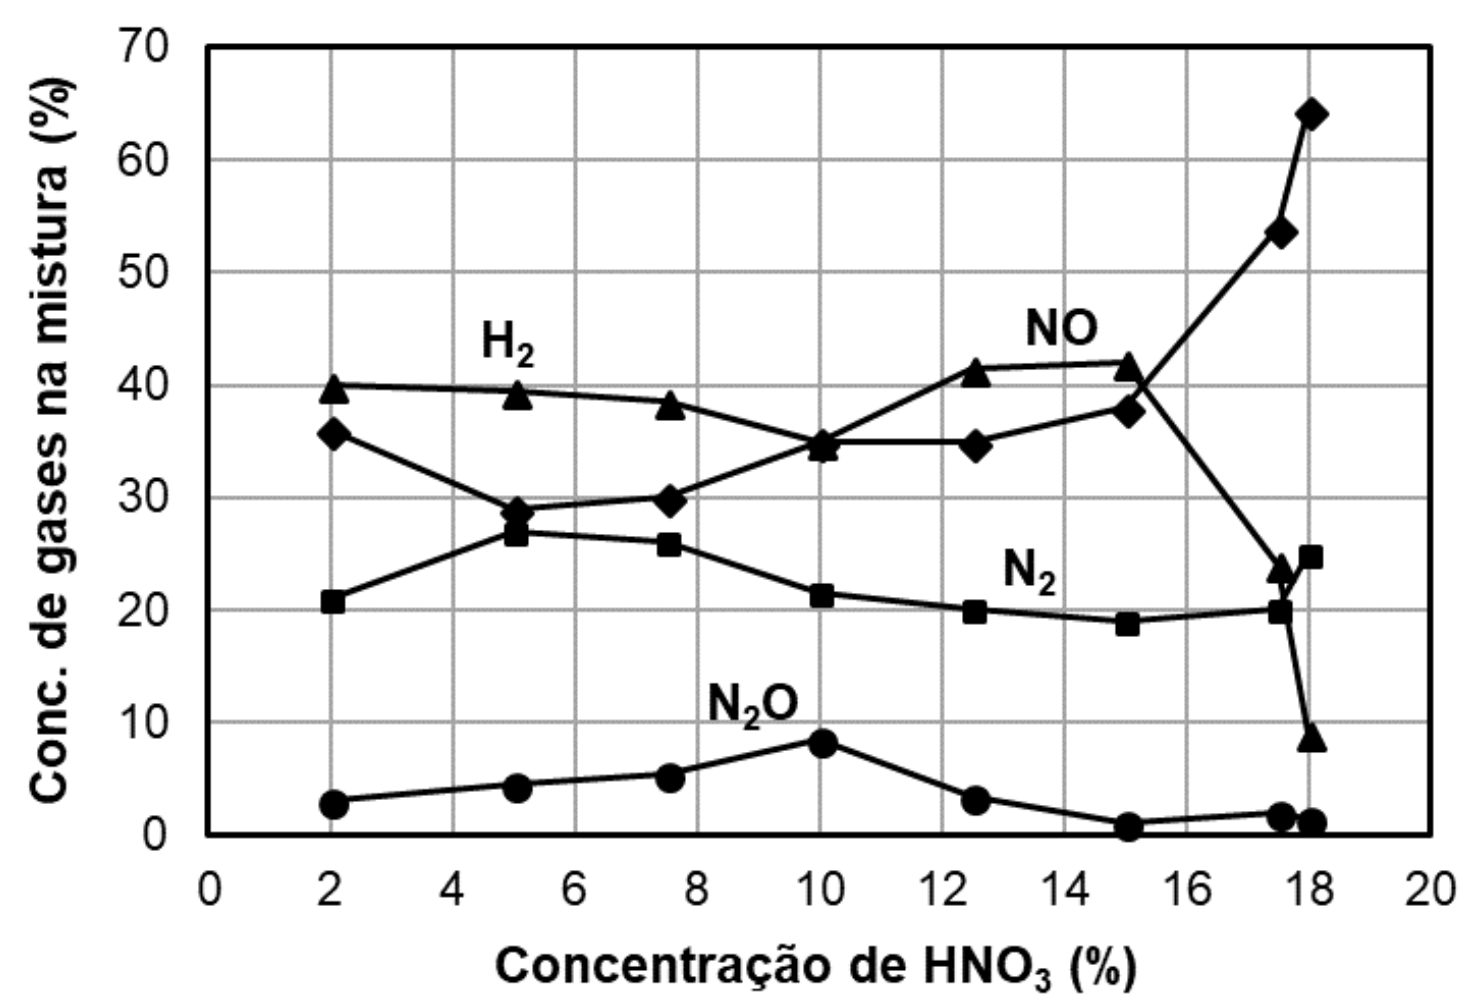
\includegraphics[width=0.5\textwidth]{figure.png}
\end{center}

Sobre as reações citadas e o gráfico mostrado, analise as afirmativas abaixo e assinale a correta:

\begin{enumerate}[label = (\alph*)]
	\item Apenas a reação de produção de \chemfig{H_2}(g) e \chemfig{N_2}(g) correspondem a reações de oxirredução.
	\item Utiliizando concentrações de ácido nítrico entre 2$\%$ e 18 $\%$, a reação que envolve a redução do nitrogênio de um número de oxidação +5 para +1 é aquela com formação de menor $\%$ de produto.
	\item Na reação, ao utilizar a concentração de 10$\%$ de ácido nítrico, pode se afirmar qua a diferença de potencial padrão da reação de produção de gás hidrogênio é igual àquele da reação de produção de monóxido de nitrogênio, uma vez que as concentrações destes gases são igual na coposição da mistura gasosa produzida.
	\item Os dados apresentados no gráfico possibilitam concluir que utilizando concentração acima de 16$\%$ de ácido nítrico a reação com a produção de \chemfig{NO} é aquela termodinamicamente mais favóravel. 
	\item Através apenas do cálculos das diferenças de potenciais padrão das reações de produção dos gases (hidrogênio, nitrogênio, monóxido de nitrogênio e óxido de dinitrogênio) pode-se prever qual ou quias os produtos termodinamicamente mais favoráveis.
\end{enumerate}
